% \chapter{Discussion} % maybe the part with automatic optimization
In the previous chapters, we have looked in broader terms at the problems we are faced with when trying to make \textit{TinyFace} a reality. In this chapter, we will look into the combination of decisions and parameter choices that have enabled us to accomplish our goal - the end to end development of a dataset generator, model training framework and \textit{TF Lite} interpreter app.

\section{The Final Dataset}
The model has then been trained on a custom generated dataset, containing data that has been scraped from the web, on a total of 30,000 images - 14,000 faces and 16,000 non-face objects - as such we have a binary classifier. Each image is \textit{100 * 100} pixels large and grayscale. Moreover, each image has been contrast-normalized to a range of 0 to 10, to minimize contrast variance, which would have otherwise been seriously impeding the model's performance during real-world use if left as it had been by default in the images (0-255). A side effect of this, it should be noted, is that the resulting training images look \textit{pitch black} to the naked eye, and we can barely make out any details if at all since there is so little detail left for the human eye to pick up on. However, it is - in this case - advantageous to have so little dynamic range, since the neural network can use its resources to learn the actual geometric shapes and patterns of the faces, instead of wasting valuable memory on learning less-relevant contrast differences (for instance, a soft shadow to the side of one's nose) or, in other words, learning \textit{shades of gray} unnecessarily. \par

\section{Optimized SqueezeNet}
When choosing which model architecture to use, color images we initially used for experiementation. However, these only really made the model size increase so drastically that the finished files could only barely fit inside the memory of the embedded device. As such, the decision was made to switch to exclusively gray-scale images. This also meant the model complexity was reduced since the convolutional layers only had to be applied to one dimension, instead of three. \par
The final model was, as previously mentioned, based on SqueezeNet. The final trained model file is \textit{139 KB} large, after having been compressed and quantified to 8-bit weights. \par
\section{The Golden Training Formula}
After repeatedly experimenting with different numbers and combinations for each of the hyperparameters, we have settled on a set of values that delivered the highest accuracy. The hyperparameters for the most successful training sessions have been set as follows: 
\begin{itemize}
    \item 5 training epochs
    \item a batch size of 32 samples
    \item a 75\%-25\% divide between training and test data
    \item a dropout rate of 10\%
\end{itemize}
The choice of hyperparameters and the evaluation of training performance is a lengthy process, and a relatively big time drain, in general, plus highly repetitive. That makes it a prime candidate for automation. A solution for this will be proposed in the next chapter. In \textit{Figure \ref{training_tf_gold}}, we can see the training accuracy of the model, as reported by TensorFlow. We have achieved 99\% accuracy several times on the training data, which means that our model really is a good fit for learning images. 

\begin{figure}
    \centering
    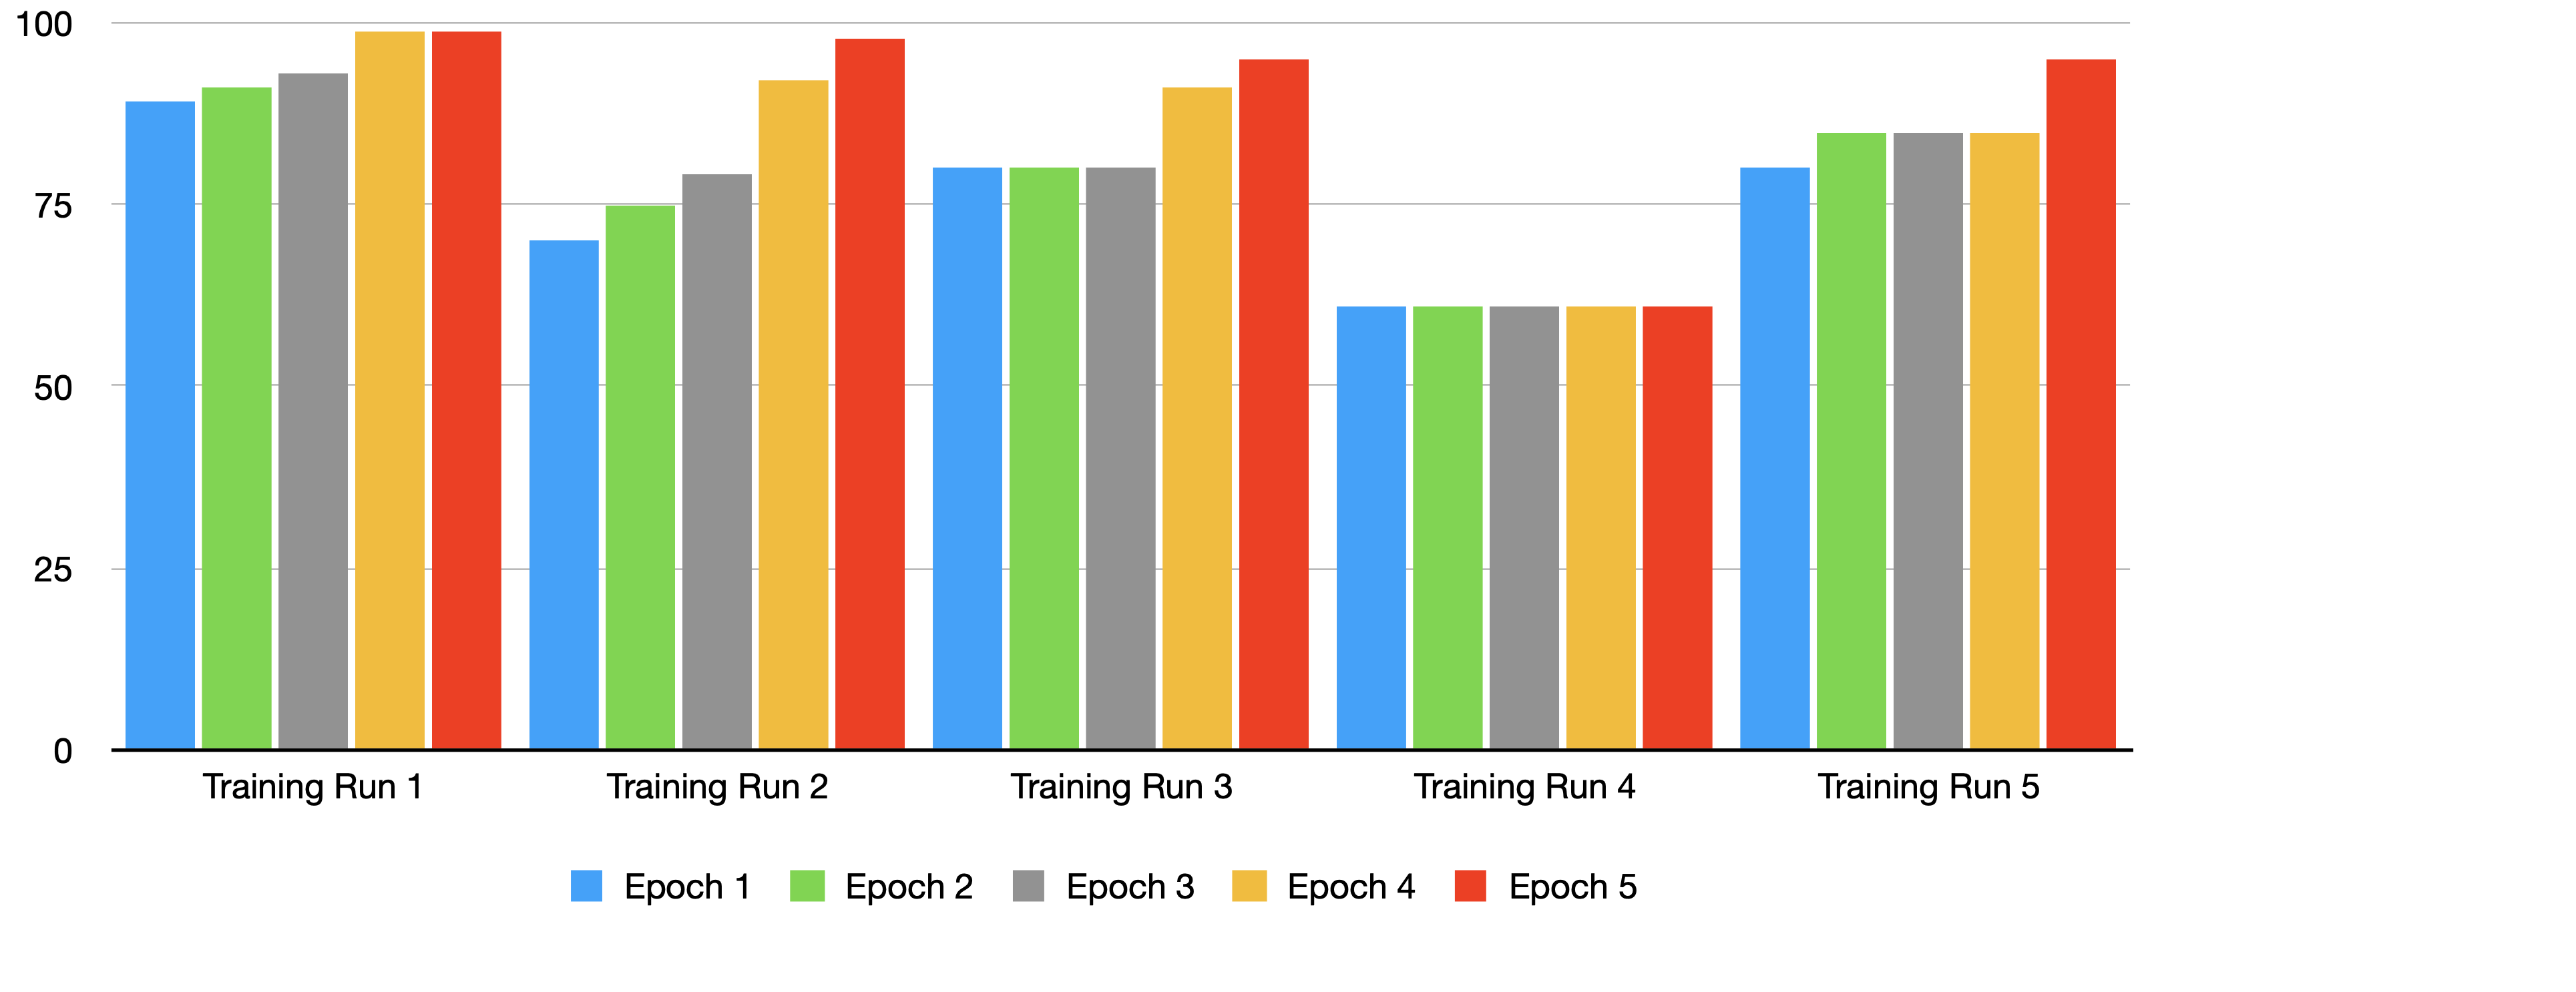
\includegraphics[width = 16 cm]{figures/training_fig1}
    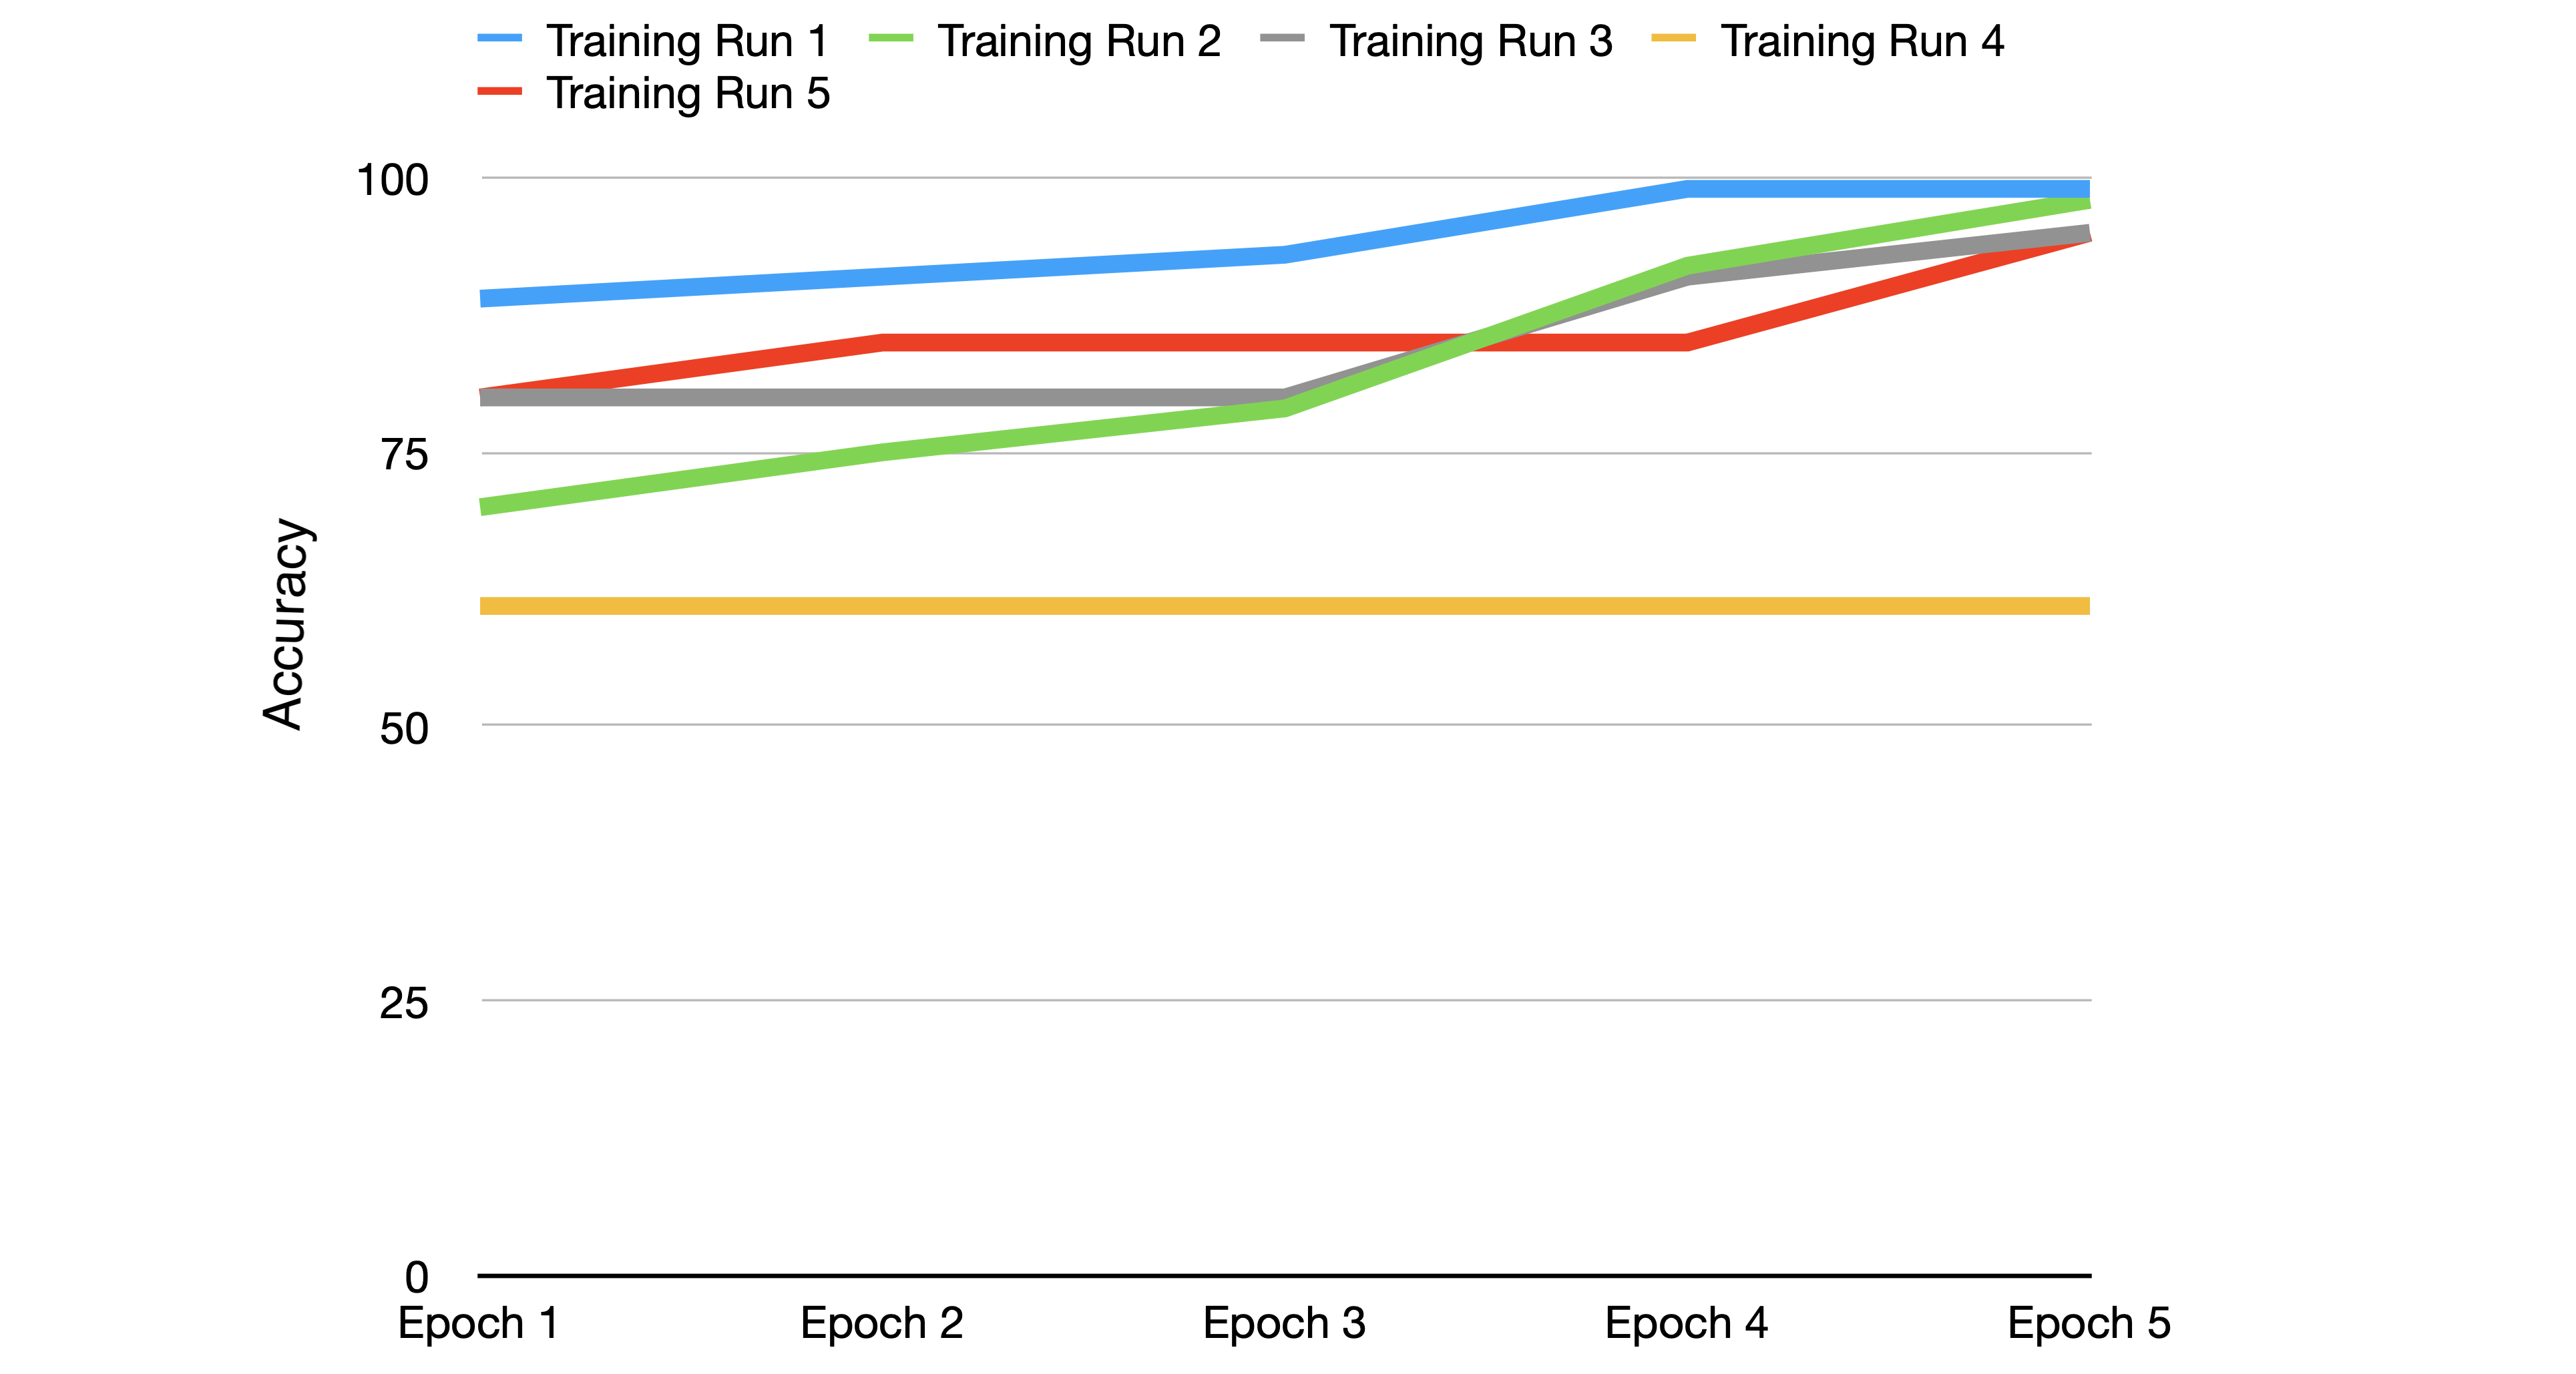
\includegraphics[width = 16 cm]{figures/training_fig2}
    \caption{Training with 5 epochs, for five different runs. During run number 4, the model failed to learn the data, and averaged out at a reported 61\%.}
    \label{training_tf_gold}
\end{figure}

\newpage
\section{Example Inference}
Let us look at five representative images of the author, that the interpreter has been called upon. We have 3 figures. In \textit{Figure \ref{webcam_orig}}, we can see the original images, as they appear to us in the \textit{live-view} of the webcam. In \textit{Figure \ref{interpreter_eyes}}, we can see what the converted images look like \textit{in the eyes of the interpreter}. In \textit{Table \ref{tab:results}}, we can see what the interpreter has determined for each image. \par
For the first image, we have a clear answer: a face. For the second image, probably because of the tilted head, we have a not-so-clear 48-51 divide between face and non-face. The third image, where even glasses are present, is a clear \textit{face}. The fourth image, where the webcam was partially covered, is a non-face object. The same is true for the last image, where the webcam has, once again, been intentionally covered.

\begin{figure*}[ht!]
    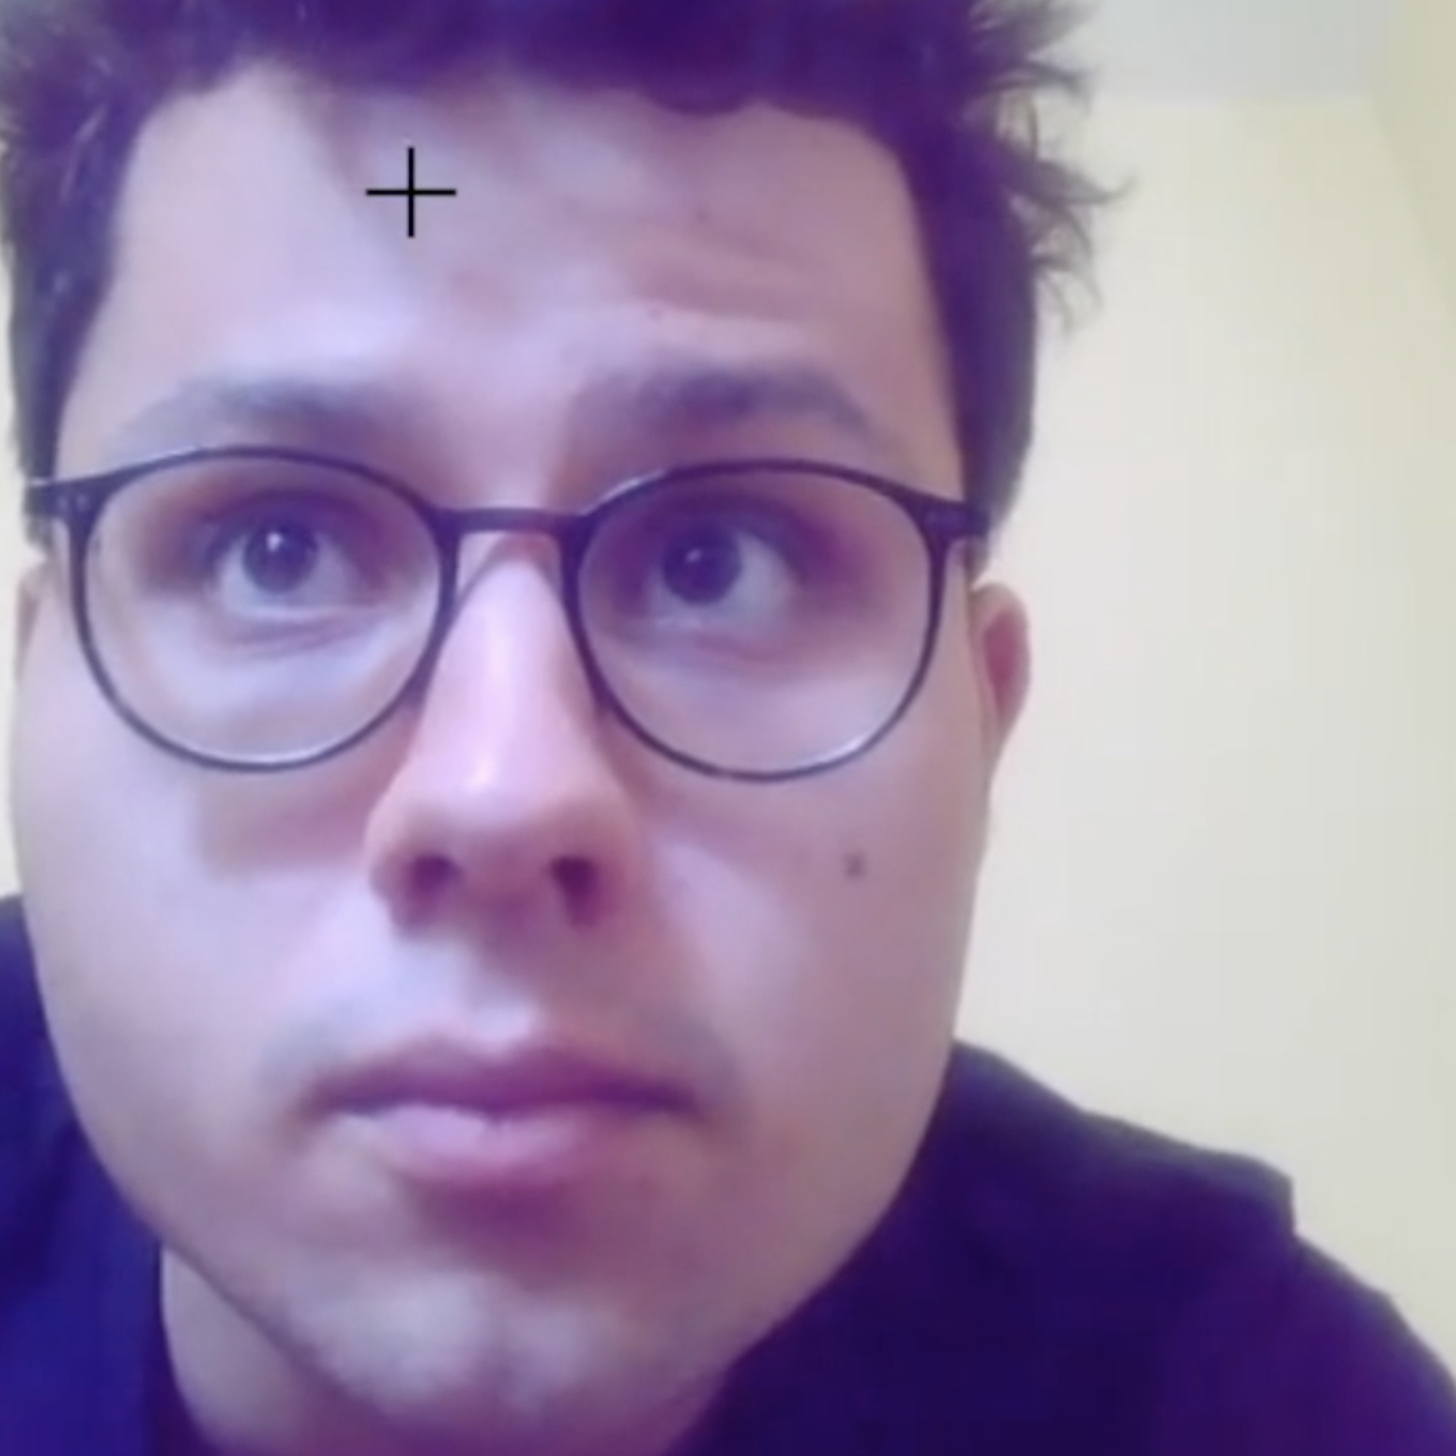
\includegraphics[width = 2.8 cm]{images/inference/63_35}\hfill
    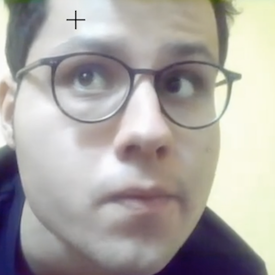
\includegraphics[width = 2.8 cm]{images/inference/48_51}\hfill
    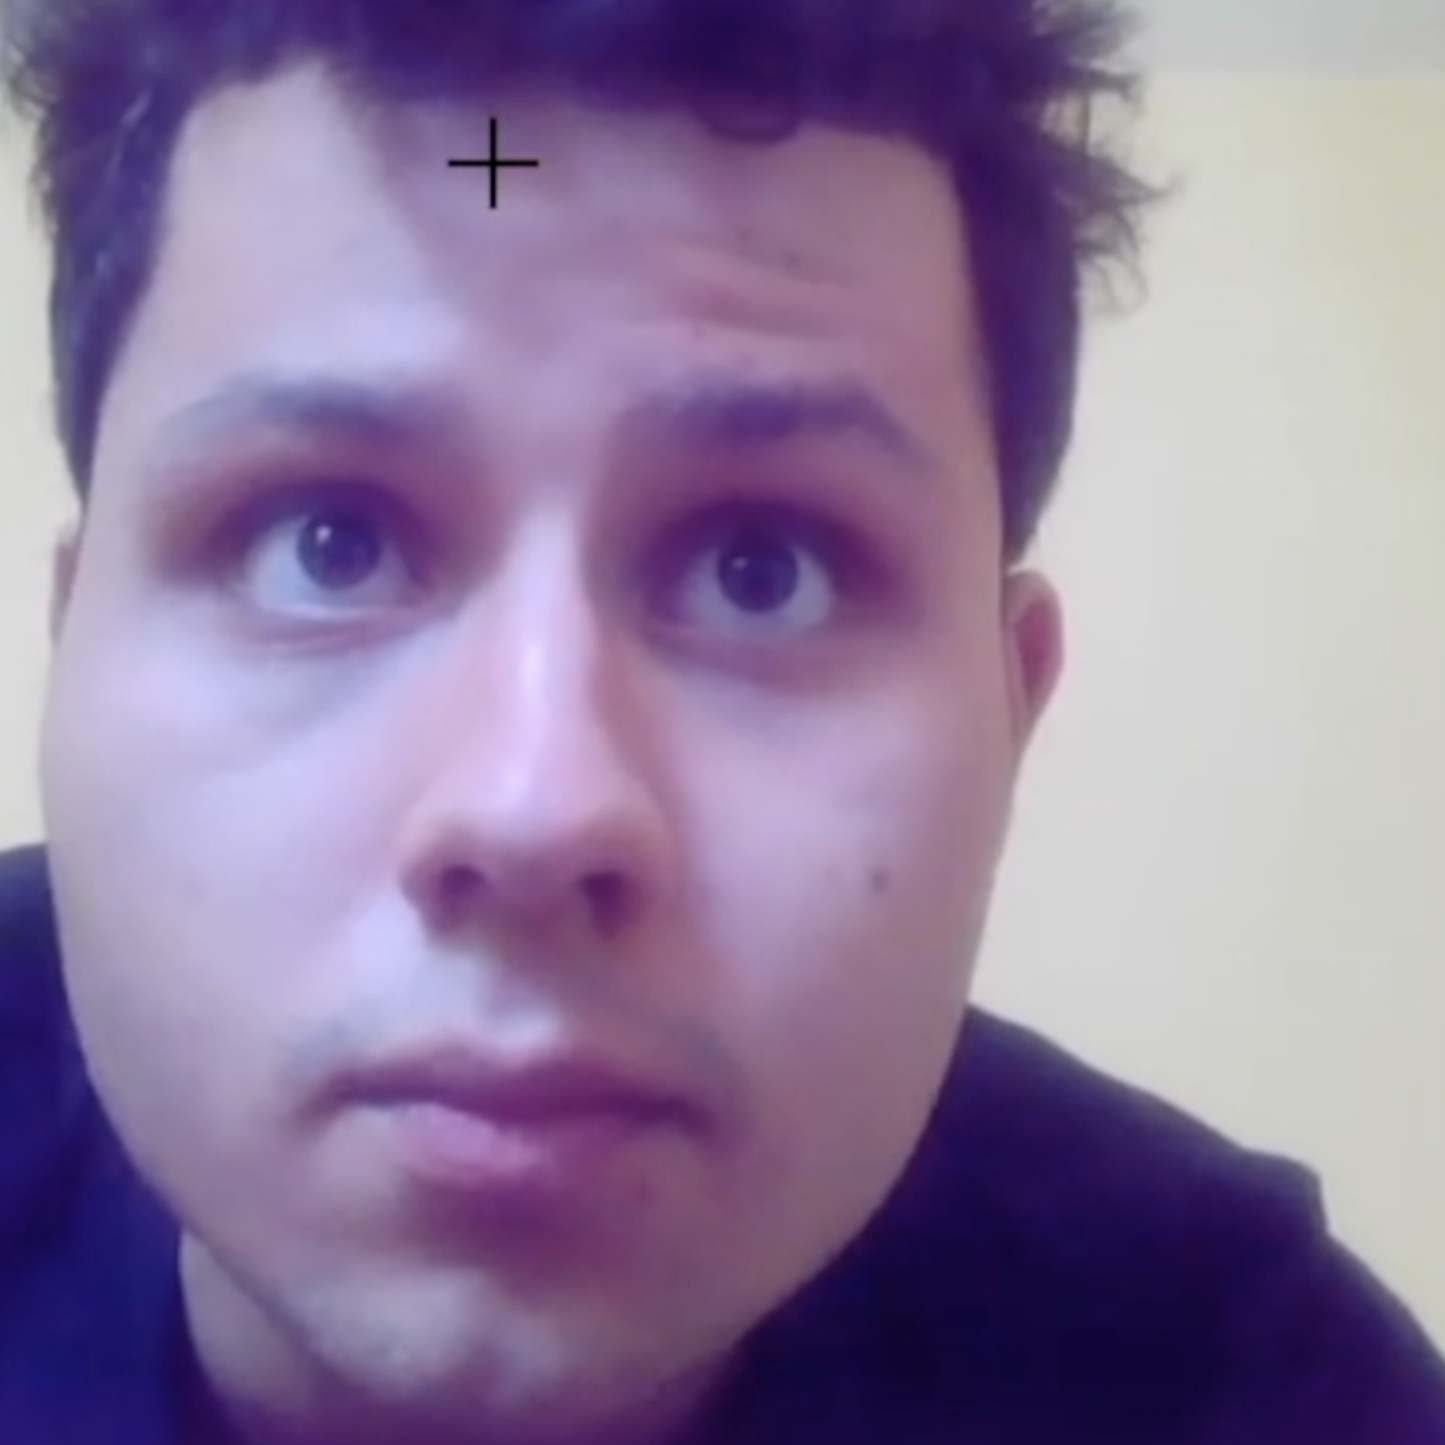
\includegraphics[width = 2.8 cm]{images/inference/61_38}\hfill
    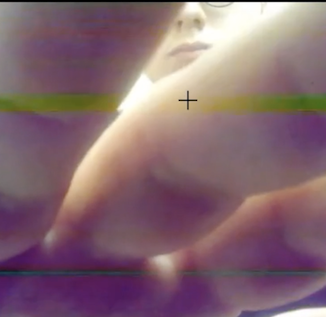
\includegraphics[width = 2.8 cm]{images/inference/41_58}\hfill
    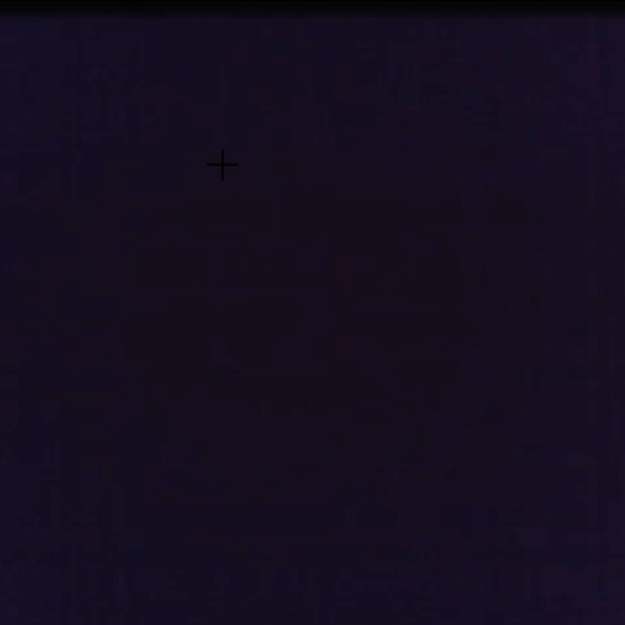
\includegraphics[width = 2.8 cm]{images/inference/37_62}\hfill
    \caption{Original images, as seen on webcam - cropped by hand to similar sizes for the sake of comparison with the images in the following figure and turned to black and white from color for consistency.}
    \label{webcam_orig}
\end{figure*}

\begin{figure*}[ht!]
    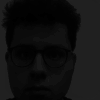
\includegraphics[width = 2.8 cm]{images/inference/frame_0}\hfill
    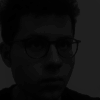
\includegraphics[width = 2.8 cm]{images/inference/frame_1}\hfill
    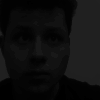
\includegraphics[width = 2.8 cm]{images/inference/frame_3}\hfill
    
\includegraphics[width = 2.8 cm]{images/inference/frame_4}\hfill
    
\includegraphics[width = 2.8 cm]{images/inference/frame_5}\hfill
    \caption{What the interpreter actually \textit{"sees"}. The images have sides of 100*100 pixels, their dynamic range has been downsampled to a value between 0 and 9 grayscale.}
    \label{interpreter_eyes}
\end{figure*}

\begin{table}
    \centering
    \begin{tabular}{|c|c|c|c|}
        \hline
        Image & \% confidence Face & \% confidence Non-Face  & Result \\ \hline
        1 & 61 \% & 38 \%  & Face \\ \hline
        2 & 48 \% & 51 \%  & No Face (it's a tie, almost)\\ \hline
        3 & 63 \% & 35 \%  & Face \\ \hline
        4 & 41 \% & 58 \%  & No Face \\ \hline
        5 & 37 \% & 62 \%  & No Face \\ \hline
    \end{tabular}
    \caption{Results of inference when the interpreter was called on the example images.}
    \label{tab:results}
\end{table}

\newpage
\section{A Longer Test}
We have also run inference for longer periods, with the faces of several people, and achieved the following results, presented in \textit{Figure \ref{fig:long_inference} and Table \ref{tab:inference_long_term}}. These other faces will not be included, since they are not the author's own. We can see that the inference was \textit{relatively} accurate in our empirical tests: often around 80\%, and this in 4 different scenarios, with 3 different people. 

\begin{figure}
    \centering
    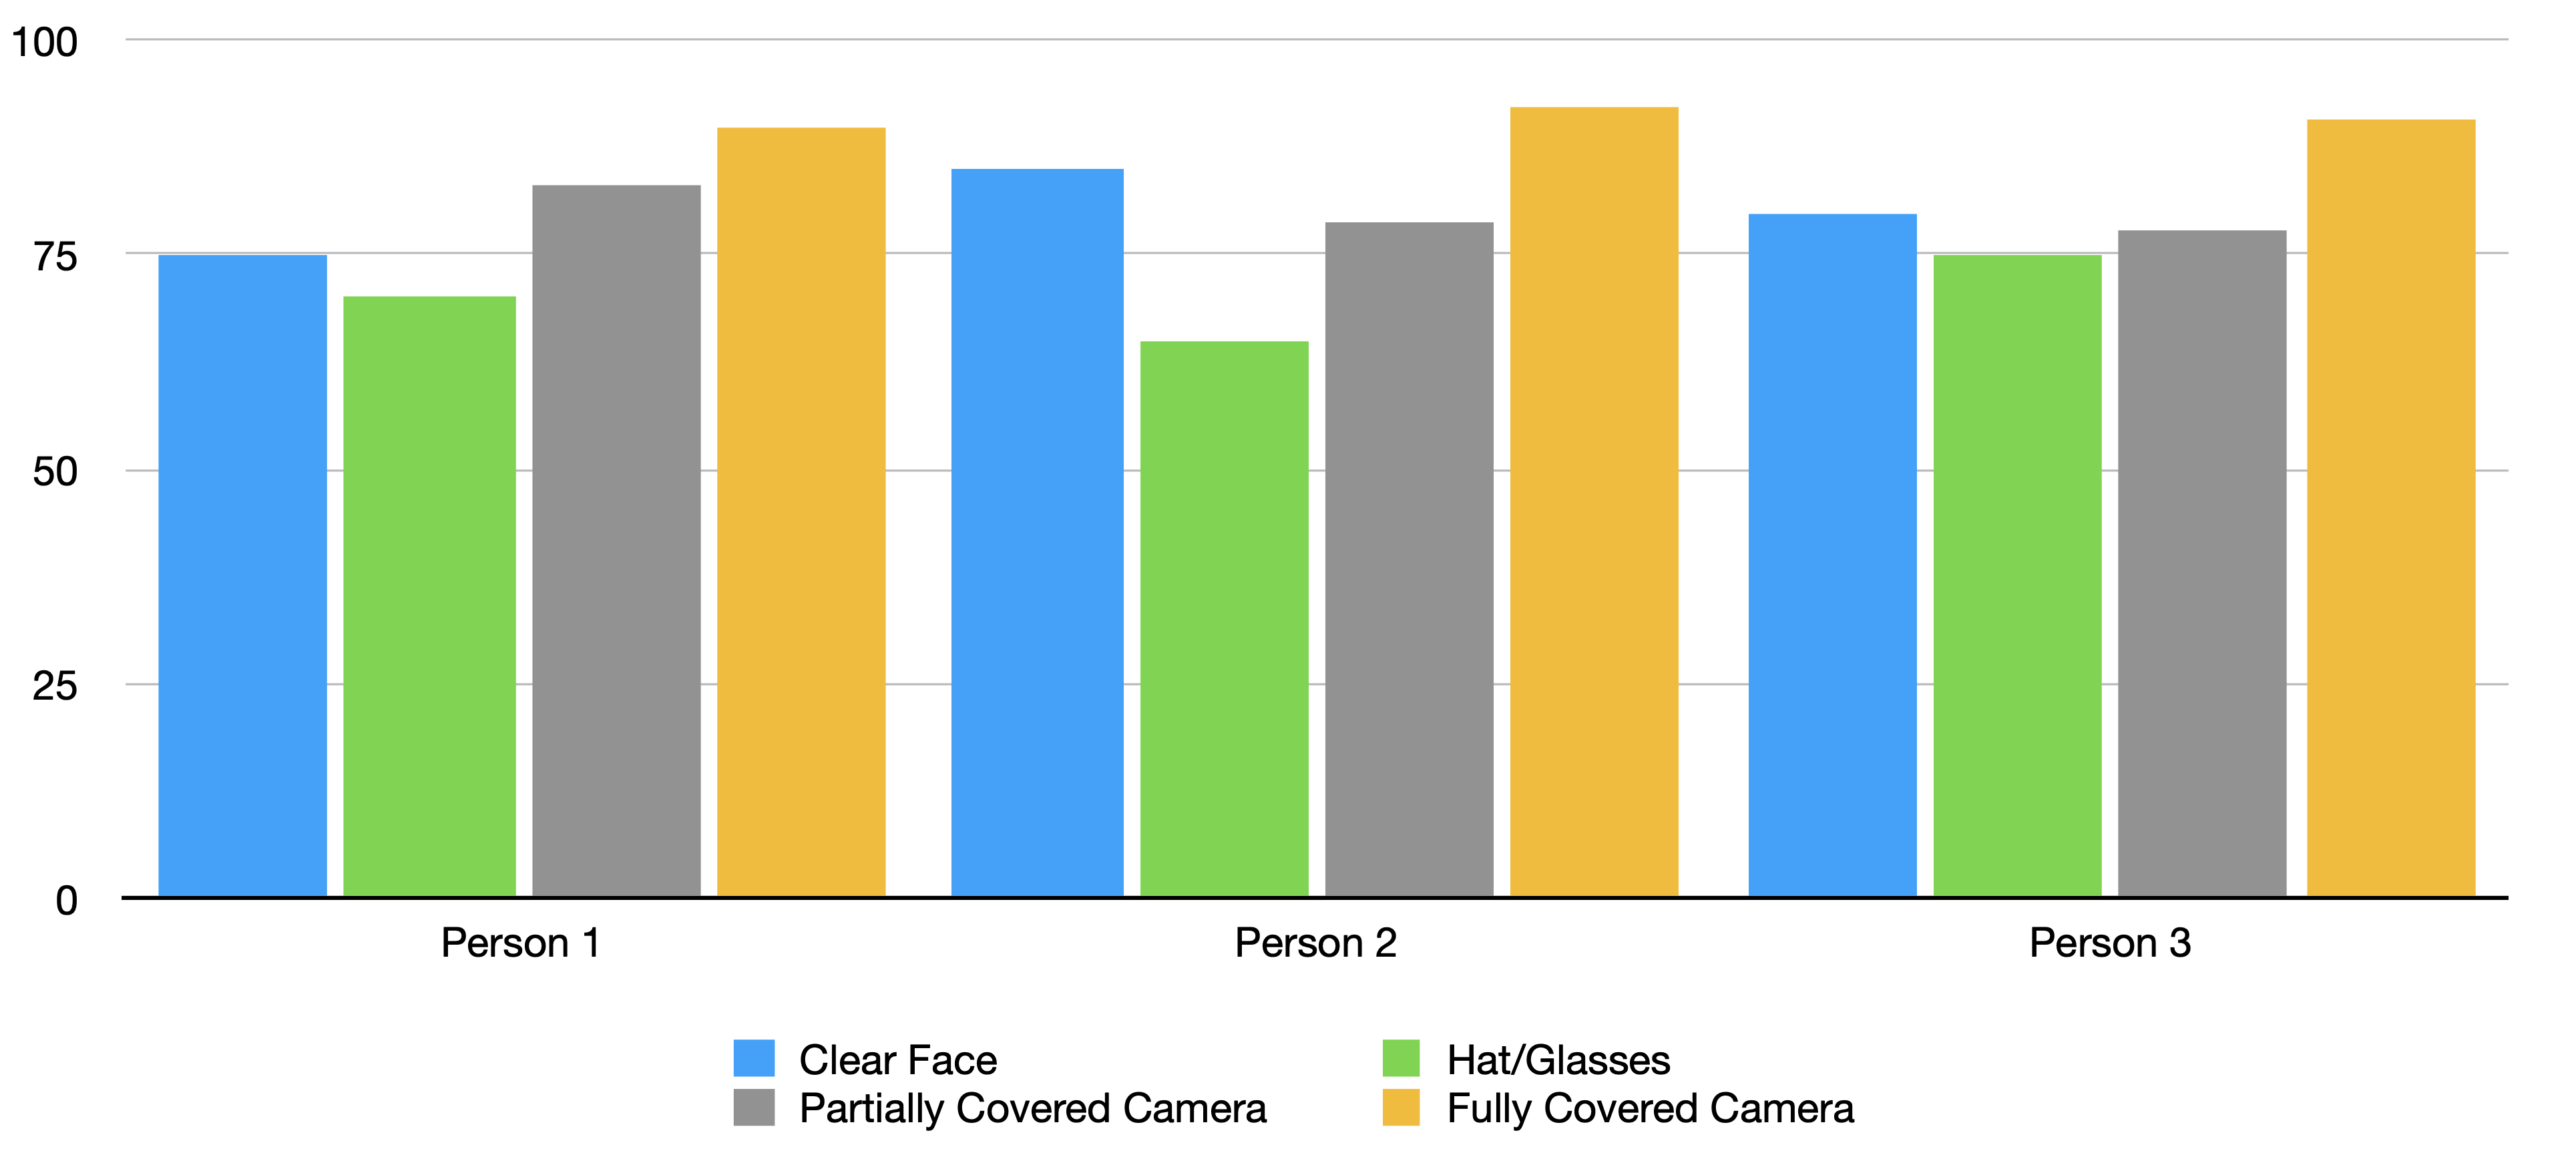
\includegraphics[height = 7 cm]{figures/inference_long_test}
    \caption{Results of another accuracy test for inference: how many of 20 images were correctly identified.}
    \label{fig:long_inference}
    \quad
\end{figure}
\begin{table}
    \centering
    \begin{tabular}{|c|c|c|c|c|}
        \hline
        Person & Clear Face & Glasses/Hat & Partially Covered Camera & Fully Covered Camera  \\ \hline
        1 & 75 \% & 70 \% & 80\% & 90 \% \\ \hline
        2 & 85 \% & 65 \% & 80\% & 90 \% \\ \hline
        3 & 80 \% & 75 \% & 80\% & 90 \% \\ \hline
    \end{tabular}
    \caption{Results from above, transcribed.}
    \label{tab:inference_long_term}
\end{table}

\section{Discussing the Results}
Let us, therefore, close this chapter by looking back at what has been achieved. We have so far presented a complete, end-to-end, process for running face detection in a TensorFlow Lite interpreter. We started out with compiling our own dataset and developing our own model architecture, then optimized size and performance, deployed to the interpreter, and evaluated performance. As such, we have created a new application of \textit{TinyML}, that we have called \textit{TinyFace}. We have achieved an accuracy level of around 80 \% or more in our empirical test, which is to be expected for models of such size on real-life benchmarks. Moreover, let us not forget that systems designers of such systems would often implement several extra safeguards at higher abstraction levels, higher up in the system, to compensate for the crude accuracy of our almost metal-level implementation of Machine Learning. \par
With this in mind, and having now accomplished what we set out to do, let us close this chapter and proceed to the final one, where we will present possible future research directions, and deliver our closing remarks.